\documentclass[a4paper]{article}

\usepackage[UTF8]{ctex}
\usepackage[a4paper,margin=1in]{geometry}
\usepackage{graphicx}
\usepackage{float}
\usepackage{listings}
% \usepackage{listings-rust}
\usepackage{longtable}
\usepackage{booktabs}
\usepackage{hyperref}
\usepackage{fancyhdr}
\usepackage{lastpage}
\usepackage{color}
\usepackage{indentfirst}        % 首段缩进
\setlength{\parindent}{2em}     % 缩进2字符
\usepackage{zhnumber}           % 中文编号
\usepackage[dvipsnames,table,xcdraw]{xcolor}
\usepackage{adjustbox}
\usepackage{subcaption}
\usepackage{amsmath}
\usepackage{amssymb}
\usepackage[many]{tcolorbox}
% \newfontfamily{\enfont}{Arial}  % 定义英文字体
\usepackage{enumitem}
\usepackage{xeCJK}
\usepackage[T1]{fontenc}
\usepackage{lmodern}
\usepackage{inconsolata} % 使用更美观的等宽字体 Inconsolata
\usepackage{multirow} % 用于表格中的多行合并
\usepackage{tikz} % 添加 TikZ 宏包用于绘制流程图
\usetikzlibrary{positioning} % 添加定位库以支持 'of' 语法

% 全局设置（影响所有级别）
\setlist[itemize]{
    itemsep=2pt,
    topsep=4pt,
    parsep=1pt,
    leftmargin=3em
}

% 仅设置第一级（最高级）
\setlist[itemize,1]{
    label=\textcolor{orange}{$\blacktriangleright$},
    font=\color{blue!80!black}\small\bfseries,
    before={\color{blue!80!black}\small\bfseries}
}

% 重置第二级及更深级别（恢复默认样式）
\setlist[itemize,2]{
    label={\normalfont\textbullet},
    font=\normalfont\normalsize\color{black},
    before={\color{black}},
    leftmargin=*
}
\setlist[itemize,3]{
    label={\normalfont$\circ$},
    font=\normalfont\normalsize,
    before={},
    leftmargin=*
}


% 定义可分页的引用环境
\newtcolorbox[auto counter]{myquote}[1][]{
    % breakable,                     % 允许跨页分断
    % enhanced jigsaw,               % 优化分页处的边框
    colback=gray!5,                % 背景色
    colframe=gray!30,              % 边框色
    left=5mm, right=5mm,           % 左右内边距
    top=3mm, bottom=3mm,           % 上下内边距
    width=0.85\textwidth,         % 宽度
    center,                     % 居中
    arc=0mm,                       % 直角边框
    boxrule=0.5pt,                 % 边框线宽
    fontupper=\small\linespread{1.1}\selectfont, % 行距微调（1.1倍）
    % fontupper=\sffamily\linespread{1.05}\selectfont, % 无衬线 + 紧凑行距
    before upper={\parindent2em\color{black!40!blue}\itshape\small\kaishu}, % 深蓝色文本
    #1 % 允许额外参数
}

%\newcommand{\college}{中山大学计算机学院}
\newcommand{\projname}{计算机网络实验|实验二}
\newcommand{\reporttitle}{网络编程}
\newcommand{\groupno}{第一组}
\newcommand{\authorname}{欧阳易芃、马福泉、刘昊、彭怡萱}
\newcommand{\major}{计算机科学与技术}
\newcommand{\adviser}{谢逸}
\newcommand{\startdate}{2025年10月1日}
\newcommand{\labenddate}{2025年10月10日}
\newcommand{\labroom}{实验D402}

\pagestyle{fancy} % 使用 fancyhdr 风格
\fancyhf{}      % 清空默认的页眉页脚

% 设置页眉
\fancyhead[L]{\kaishu \projname}      % 左侧页眉显示项目名称
\fancyhead[C]{\kaishu \reporttitle}    % 中间页眉显示报告标题
\fancyhead[R]{\kaishu \authorname} % 右侧页眉显示作者姓名

% 设置页脚
\fancyfoot[C]{第 \thepage 页，共 \pageref{LastPage} 页} % 中间页脚显示页码

% 去除页眉页脚与正文之间的分隔线
\renewcommand{\headrulewidth}{0.4pt}
\renewcommand{\footrulewidth}{0pt}

% 设置文档背景颜色
\definecolor{mybgcolor}{RGB}{0, 0, 0} % 定义背景颜色
\definecolor{NavyBlue}{RGB}{0,0,128} % 添加颜色定义



% 全局设置lstlisting的样式
\lstset{
    language=C, % 设置默认语言
    basicstyle=\footnotesize\ttfamily, % 设置字体族
    breaklines=true, % 自动换行
    keywordstyle=\bfseries\color{blue}, % 设置关键字为粗体，颜色为蓝色
    morekeywords={}, % 设置更多的关键字，用逗号分隔
    emph={}, % 指定强调词，如果有多个，用逗号隔开
    emphstyle=\bfseries\color{Rhodamine},
    commentstyle=\itshape\color{green!50!black},
    stringstyle=\bfseries\color{PineGreen!90!black},
    columns=fullflexible,% 设置列宽
    numbers=left,
    numbersep=2em,
    numberstyle=\footnotesize\color{gray},
    frame=single,
    framesep=1em,
    showstringspaces=false,% % 不显示字符串中的空格
    keepspaces=true,
    backgroundcolor=\color{gray!5},
    % linewidth=0.8\linewidth, % 设置宽度为当前行宽的 80%
    xleftmargin=0.2\linewidth, % 左右边距自动调整
    xrightmargin=0.08\linewidth,
    % gobble=2, % 可选：移除代码前的缩进
    % postbreak=\mbox{\textcolor{red}{$\hookrightarrow$}\space}, % 可选：换行符样式
    captionpos=b, % 可选：标题位置
    aboveskip=1em, % 可选：上方间距
    belowskip=1em, % 可选：下方间距
}

\begin{document}


% 封面
\begin{titlepage}
    \centering
    
    
\includegraphics[width=10cm]{img/SYSULogo.png}

    \vspace{1em}
    %{\Large \college \par}
    \vspace{1em}
    {\Large \kaishu \projname \par}
    \vspace{3em}

    {\fontsize{40pt}{42pt}\kaishu \selectfont \boldmath \reporttitle\par}
    \vspace*{\fill}

    \begin{center}
    {\Large
    \makebox[5em][s]{小组编号}:\underline{\makebox[15em][c]{\kaishu \groupno}}\\[1em]
    \makebox[5em][s]{组员姓名}:\underline{\makebox[15em][c]{\kaishu 欧阳易芃、马福泉}}\\[0.5em]
    \makebox[5em][s]{} \underline{\makebox[15em][c]{\kaishu 刘昊、彭怡萱}}\\[1em]
    \makebox[5em][s]{专业}:\underline{\makebox[15em][c]{\kaishu \major}}\\[1em]
    \makebox[5em][s]{课程教师}:\underline{\makebox[15em][c]{\kaishu \adviser}}\\[1em]
    \makebox[5em][s]{起始日期}:\underline{\makebox[15em][c]{\kaishu \startdate}}\\[1em]
    \makebox[5em][s]{结束日期}:\underline{\makebox[15em][c]{\kaishu \labenddate}}\\[1em]
    \makebox[5em][s]{实验地点}:\underline{\makebox[15em][c]{\kaishu \labroom}}
    }
    \end{center}

    \vspace*{\fill}
\end{titlepage}

% 目录
\tableofcontents
\newpage

\section{实验概述}

\subsection{实验目标}
\begin{itemize}
    \item 连接实验设备、完成主机地址配置
    \item 基于套接字编程实现端到端的UDP通信(1inux或windows)
    \item 发送端连续发送100个UDP数据包，在接收端统计丢失的数据包在实验时，运行wireshark，对通信中的数据包进行跟踪分析
\end{itemize}

\paragraph{提示：}

\begin{itemize}
    \item 套接字编程方法可以参考网上的方法，也可以参考本文件夹中的附件。
    \item 编程方法不限，但要求达到实验目的。
    \item 可以关闭防火墙
\end{itemize}

\begin{figure}[H]
    \centering
    \adjustbox{
        max width=0.8\linewidth,
        max height=0.6\textheight,
        min width=1cm,
        min height=1cm,
        keepaspectratio
    }{
        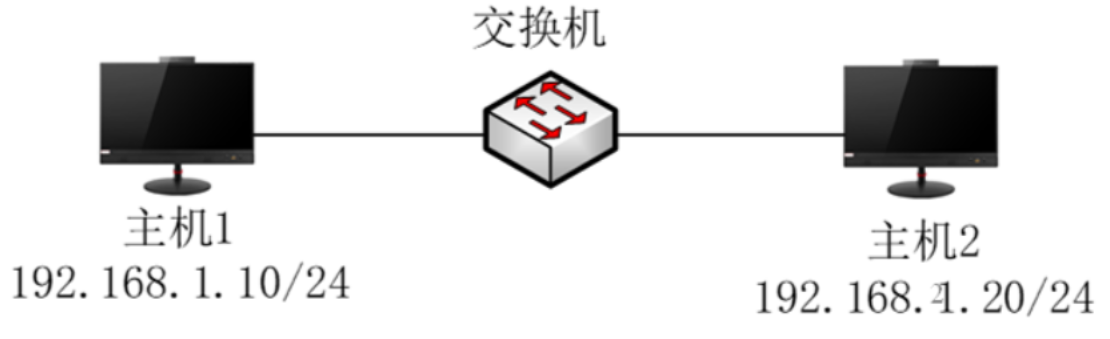
\includegraphics{img/target_connection.png}
    }
    \caption{连接示意图}
\end{figure}

\subsection{实验思考}
\begin{itemize}
    \item 说明在实验过程中遇到的问题和解决方法
    \item 给出程序详细的流程图和对程序关键函数的详细说明。
    \item 使用SocketAPI开发通信程序中的客户端程序和服务器程序时,各需要哪些不同 的函数?
    \item 解释connect()、bind()等函数中struct sockaddr*addr参数各个部分的含义并用具体的数据举例说明。
    \item 说明面向连接的客户端和面向非连接的客户端在建立Socket时有什么区别
    \item 说明面向连接的客户端和面向非连接的客户端在收发数据时有什么区别。面向非 连接的客户端又是如何判断数据发送结束的?
    \item 比较面向连接的通信和无连接通信,它们各有什么优点和缺点?适合在哪种场合下使用?
    \item 实验过程中使用Socket时是工作在阻塞方式还是非阻塞方式?通过网络检索阐 述这两种操作方式的不同。
    \item 注意实验时简述实验思路
    \item 引起UDP数据包丢失的原因有哪些?如何解决？
\end{itemize}




\newpage

\section{实验步骤与结果}

\subsection{【任务一】连接实验设备}

根据前几次课对于交换机、路由器的熟悉，我们将主机2和3连接交换机上靠后的两个口（网线上标注了PC编号）：

\begin{figure}[H]
    \centering
    \adjustbox{
        max width=0.8\linewidth,
        max height=0.6\textheight,
        min width=1cm,
        min height=1cm,
        keepaspectratio
    }{
        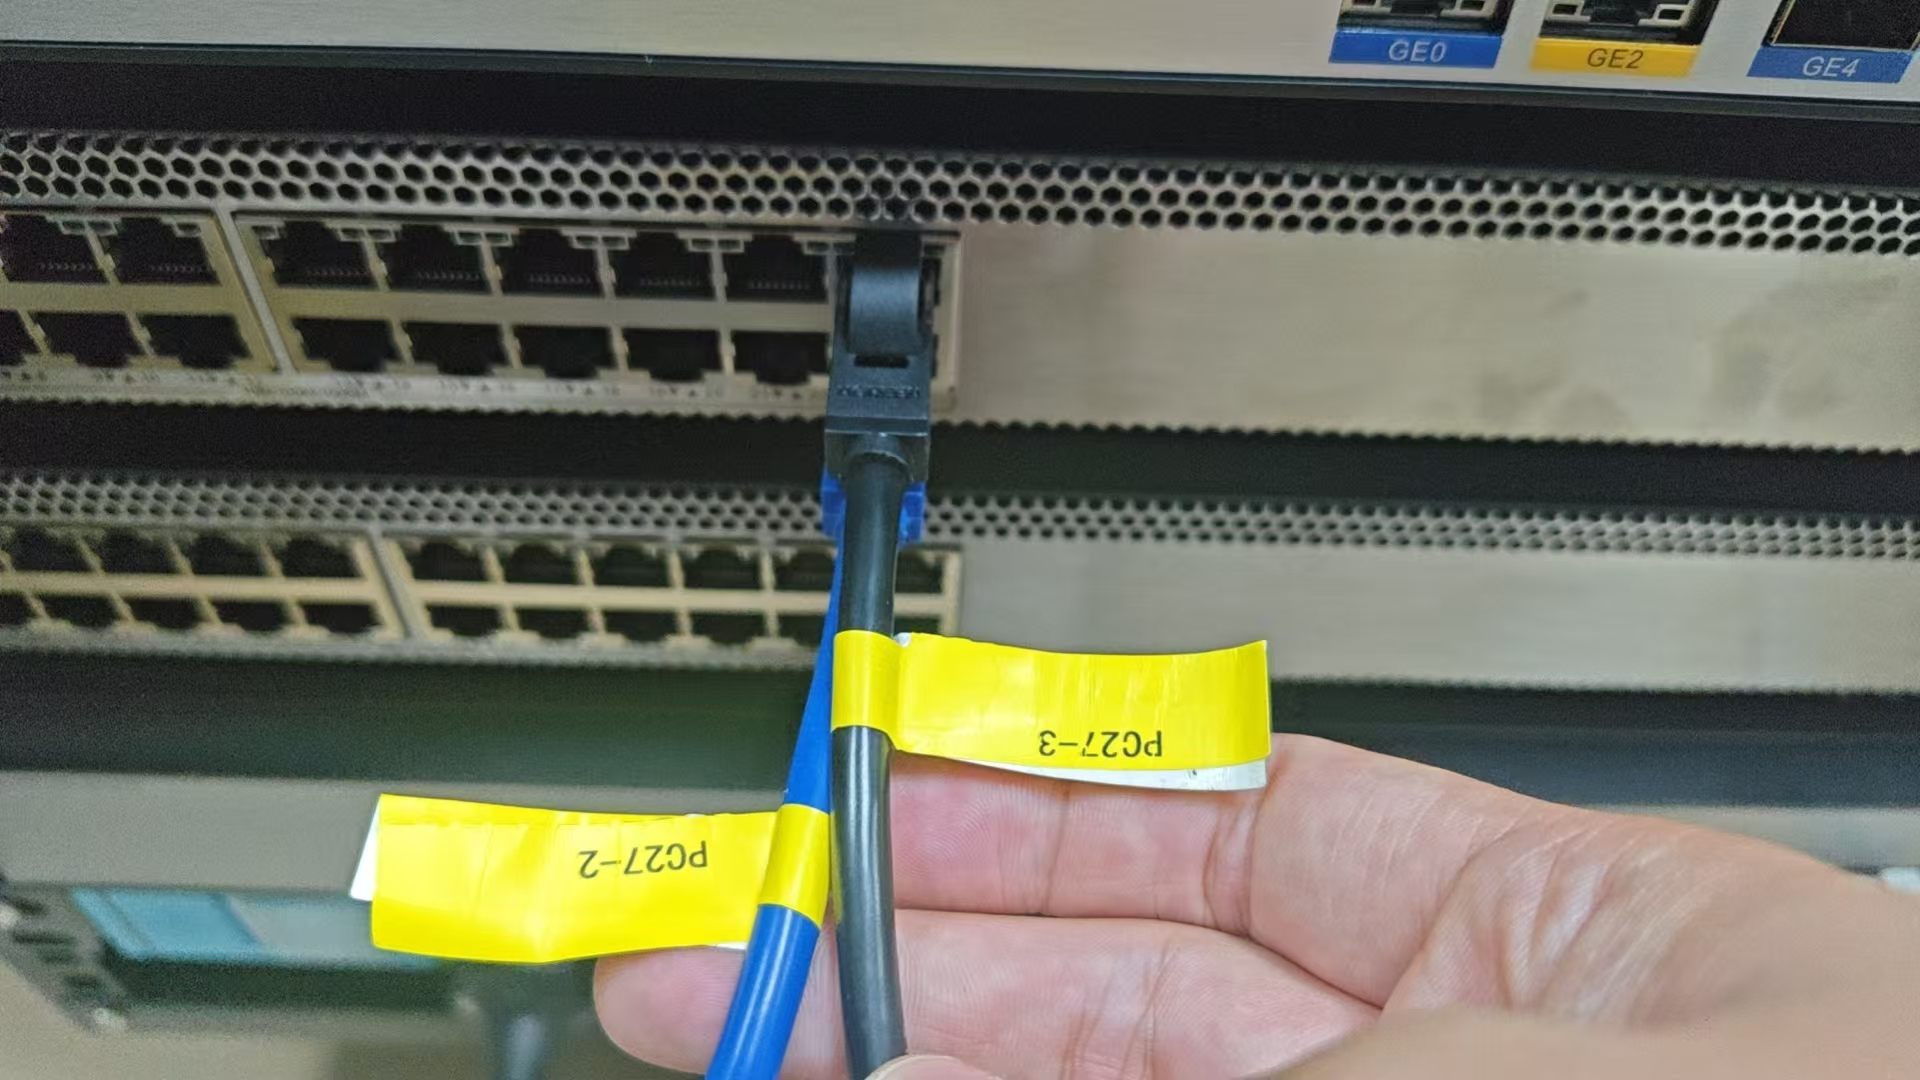
\includegraphics{img/2and3.jpg}
    }
    \caption{主机2和3连接交换机}
\end{figure}

根据上次实验ppt中给出的ip地址编号规则，我们组的主机2、3的ip地址分别是172.16.27.2和172.16.27.3。

打开两台电脑并分别尝试ping对方的ip地址，发现均能ping通，说明两台电脑已经成功连接：

\begin{figure}[H]
    \centering
    % 第一张图片
    \begin{minipage}[t]{0.48\textwidth}
        \centering
        \adjustbox{
            max width=1.05\linewidth,
            max height=0.45\textheight,
            min width=1cm,
            min height=1cm,
            keepaspectratio
        }{
            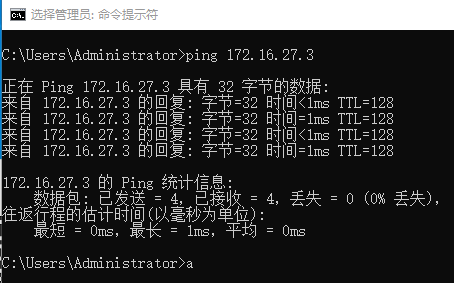
\includegraphics{img/ping2_3.png}
        }
        \subcaption{2号机ping3号机}
    \end{minipage}
    \hfill
    % 第二张图片
    \begin{minipage}[t]{0.48\textwidth}
        \centering
        \adjustbox{
            max width=1\linewidth,
            max height=0.45\textheight,
            min width=1cm,
            min height=1cm,
            keepaspectratio
        }{
            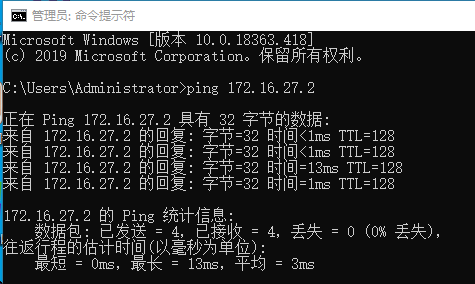
\includegraphics{img/ping3_2.png}
        }
        \subcaption{3号机ping2号机}
    \end{minipage}
    \caption{检查连接}
\end{figure}

















\subsection{【任务二】编写UDP通信程序}

根据实验要求，我们应该要分别写一个发送端程序和一个接收端程序。但主要问题在于，我们之前并没有接触过socket编程，所以首先打开课件里的介绍和代码，进行学习。

\subsubsection{学习socket编程}

根据课件\cite{ref1}和csdn的一篇详细资料\cite{ref3}，我们大概理解了socket作为应用层和传输层接口的作用：

\begin{figure}[H]
    \centering
    \adjustbox{
        max width=0.8\linewidth,
        max height=0.6\textheight,
        min width=1cm,
        min height=1cm,
        keepaspectratio
    }{
        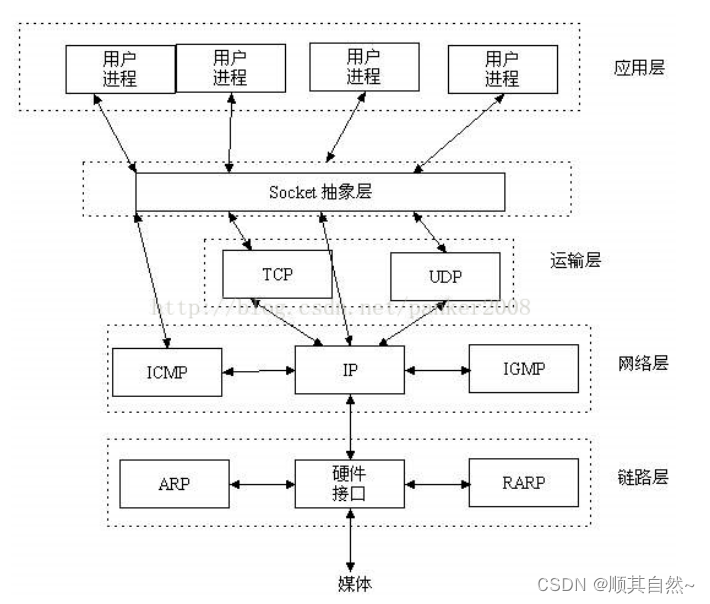
\includegraphics{img/socket_layer.png}
    }
    \caption{Socket在网络协议栈中的位置}
\end{figure}

在tcp/ip协议中，tcp三次握手建立连接，而socket也是参考tcp的连接方式，需要3次握手。在网上也找到了大神画的一个好图：

\begin{figure}[H]
    \centering
    \adjustbox{
        max width=0.8\linewidth,
        max height=0.6\textheight,
        min width=1cm,
        min height=1cm,
        keepaspectratio
    }{
        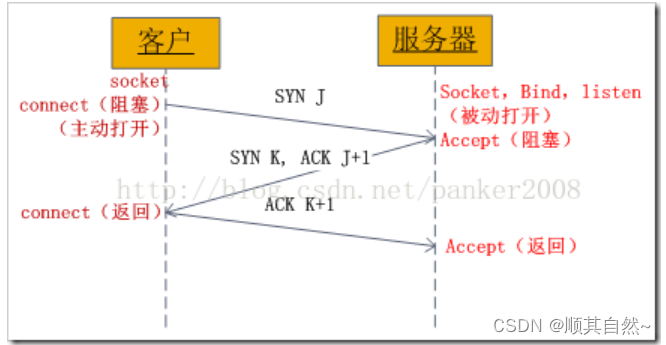
\includegraphics{img/socket_handshake.png}
    }
    \caption{Socket三次握手}
\end{figure}

具体过程的话，首先是通信的一方(被动方，称为服务器)监听某个端口，然后通信的另一方(主动方，称为客户端)试图对服务器端发送请求建立连接。该连接请求包含：服务器IP地址，服务器端口号，客户IP地址,客户端口号。

由于客户端口号由客户端的系统(TCP进程)自动选取一个当前未用的端口，这个四元组便可以在因特网中唯一标识一个逻辑连接。如果服务器收到客户端来的连接请求后，便发出响应建立该连接，这样就建立了一条逻辑信道连接，这样就建立了一条逻辑信道连接。

而课件中有对Winsock的介绍，开发过程类似文件操作，也是一个专有数据结构。而它的主要函数使用过程大概如下图：

\begin{figure}[H]
    \centering
    \adjustbox{
        max width=0.8\linewidth,
        max height=0.6\textheight,
        min width=1cm,
        min height=1cm,
        keepaspectratio
    }{
        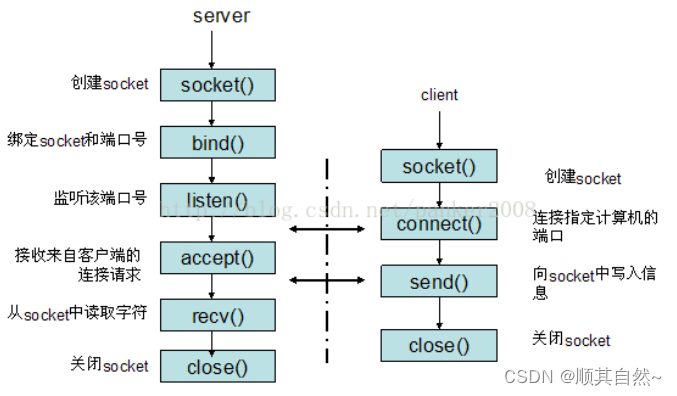
\includegraphics{img/communication_process.png}
    }
    \caption{通信过程}
\end{figure}

有了这些知识，再对照课件里面的详细函数和过程解释，我们就着手编写程序。

\subsubsection{编写发送端程序}

结合网络资料、课件和ai辅助，我们完成了程序的编写。现在拆解代码每个部分的作用：

\paragraph{头文件和宏定义：}在最前面，包含winsock2，并链接ws2\_32.lib库（这是windows下socket编程的标准库）。因为我们的发送端在3号机，所以DEST\_IP设置为2号机的ip。端口号可以随意设置一个不冲突的端口号，这里设置为8888。PACKET\_COUNT表示要发送的数据包数量，SEND\_DELAY表示发送每个包之间的延迟（毫秒），可调整以模拟网络状况。

\paragraph{初始化Winsock：}在定义好WSADATA结构和SOCKET等变量后，就要调用WSAStartup()函数初始化Winsock库，如果失败则输出错误并退出（后面很多地方用了相似的错误处理结构，不再赘述），这里MAKEWORD(2,2)表示请求使用Winsock 2.2版本。

\paragraph{创建UDP socket：}然后我们就调用socket()函数创建一个UDP套接字，参数AF\_INET表示IPv4，用SOCK\_DGRAM表示UDP协议。

\paragraph{设置目标地址：}接着我们要设置目标地址结构体destAddr，指定目标地址族为AF\_INET，端口号为8888（用htons转换为网络字节序），IP地址为2号机的ip（用inet\_addr转换）。

\paragraph{发送数据包：}然后进入循环，准备发送100个数据包。每次循环中，我们将当前包的ID（i）拷贝到发送缓冲区sendBuf的开头，这样接收端就能通过解析前4个字节知道这是第几个包。然后调用sendto()函数发送数据包，如果发送成功则打印发送的包ID，否则打印错误信息。为了避免网络拥塞，我们在每次发送后调用Sleep()函数延迟10毫秒。

\paragraph{清理资源：}发送完所有包后，打印提示信息，然后关闭套接字并调用WSACleanup()清理Winsock资源。最后等待用户按键后退出程序（这一步很重要，最开始忘了加，程序运行完就直接退出了，根本看不到结果）。

\begin{lstlisting}[language=C]
#include <stdio.h>
#include <winsock2.h>
#include <windows.h>
#pragma comment(lib, "ws2_32.lib") // 链接Winsock库
#define DEST_IP "172.16.27.2"   // 接收端的IP地址
#define DEST_PORT 8888          // 接收端的端口号，必须与接收端程序一致
#define PACKET_COUNT 100        // 要发送的数据包数量
#define SEND_DELAY 10           // 发送每个包之间的延迟（毫秒）
int main() {
    WSADATA wsaData;
    SOCKET sendSocket;
    struct sockaddr_in destAddr;
    int i;
    char sendBuf[1024];
    int packetID;

    // 初始化Winsock
    if (WSAStartup(MAKEWORD(2, 2), &wsaData) != 0) {
        printf("WSAStartup failed with error %d\n", WSAGetLastError());
        return 1;
    }

    // 创建UDP socket
    sendSocket = socket(AF_INET, SOCK_DGRAM, IPPROTO_UDP);
    if (sendSocket == INVALID_SOCKET) {
        printf("socket() failed with error %d\n", WSAGetLastError());
        WSACleanup();
        return 1;
    }

    // 设置目标地址（接收端）
    destAddr.sin_family = AF_INET;
    destAddr.sin_port = htons(DEST_PORT);
    destAddr.sin_addr.s_addr = inet_addr(DEST_IP); // 接收端的IP

    printf("Sender is ready. Sending %d packets to %s:%d...\n", PACKET_COUNT, DEST_IP, DEST_PORT);

    for (i = 1; i <= PACKET_COUNT; i++) {
        packetID = i;
        // 将包ID（一个整数）拷贝到发送缓冲区的开头
        // 这样接收端可以通过解析前4个字节来知道这是第几个包
        memcpy(sendBuf, &packetID, sizeof(packetID));

        // 发送数据包
        if (sendto(sendSocket, sendBuf, sizeof(packetID), 0, (SOCKADDR*)&destAddr, sizeof(destAddr)) == SOCKET_ERROR) {
            printf("sendto() failed for packet %d with error %d\n", i, WSAGetLastError());
        } else {
            printf("Sent packet with ID: %d\n", i);
        }

        // 短暂延迟，避免洪水式发送导致网络或接收端处理不过来
        Sleep(SEND_DELAY);
    }

    printf("\nAll packets sent.\n");

    // 清理
    closesocket(sendSocket);
    WSACleanup();

    printf("Press any key to exit...\n");
    getchar();
    return 0;
}
\end{lstlisting}

\subsubsection{编写接收端程序}

这里开头跟发送端类似，但可以看出变量多了几个，主要是为了记录收到的包ID和统计丢包情况。而前面其他部分一直到绑定端口都类似，不再赘述。

\paragraph{设置接收超时时间：}这里我们调用setsockopt()函数设置接收超时时间为5秒，这样如果5秒内没有收到任何数据，recvfrom()函数就会返回，避免程序永远阻塞。不过其实我们也发现5秒有点短了，经常两边机子会没准备好，但如果太长又会等很久，所以这里先保持设置5秒。

\paragraph{接收数据包：}然后进入一个无限循环，调用recvfrom()函数接收数据包。如果recvfrom()返回SOCKET\_ERROR，我们检查错误码，如果是WSAETIMEDOUT，说明5秒内没有收到数据，我们打印提示并跳出循环结束接收；否则打印错误信息继续等待下一个包。

如果成功接收到数据，我们检查接收长度是否至少包含一个整数（4字节），然后从缓冲区前4个字节提取包ID，并标记该包已收到。这里我们用一个数组receivedPackets来记录收到的包，索引对应包ID，值为1表示收到，0表示未收到。

\paragraph{统计丢包情况：}当退出接收循环后，我们遍历receivedPackets数组，统计哪些包未收到，并打印丢失的包ID，最后计算并打印总的丢包数和丢包率。


\begin{lstlisting}
#include <stdio.h>
#include <winsock2.h>
#include <windows.h>

#pragma comment(lib, "ws2_32.lib") // 链接Winsock库

#define RECV_PORT 8888 // 接收端监听的端口号，可以自行修改
#define PACKET_COUNT 100 // 期望接收的数据包总数

int main() {
    WSADATA wsaData;
    SOCKET recvSocket;
    struct sockaddr_in recvAddr, senderAddr;
    int senderAddrSize = sizeof(senderAddr);
    int recvLen;
    char recvBuf[1024];
    int receivedPackets[PACKET_COUNT + 1] = {0}; // 数组用于标记收到的包，索引从1到100
    int i, lostCount = 0;
    int packetID;

    // 初始化Winsock
    if (WSAStartup(MAKEWORD(2, 2), &wsaData) != 0) {
        printf("WSAStartup failed with error %d\n", WSAGetLastError());
        return 1;
    }

    // 创建UDP socket
    recvSocket = socket(AF_INET, SOCK_DGRAM, IPPROTO_UDP);
    if (recvSocket == INVALID_SOCKET) {
        printf("socket() failed with error %d\n", WSAGetLastError());
        WSACleanup();
        return 1;
    }

    // 绑定接收端的地址和端口
    recvAddr.sin_family = AF_INET;
    recvAddr.sin_port = htons(RECV_PORT);
    recvAddr.sin_addr.s_addr = htonl(INADDR_ANY); // 监听所有网络接口

    if (bind(recvSocket, (SOCKADDR*)&recvAddr, sizeof(recvAddr)) == SOCKET_ERROR) {
        printf("bind() failed with error %d\n", WSAGetLastError());
        closesocket(recvSocket);
        WSACleanup();
        return 1;
    }

    printf("Receiver is running on 172.16.27.2:%d...\nWaiting for packets...\n", RECV_PORT);

    // 设置超时时间（5秒）
    // 如果5秒内没有收到任何数据，recvfrom将返回，避免程序永远阻塞
    DWORD timeout = 5000;
    setsockopt(recvSocket, SOL_SOCKET, SO_RCVTIMEO, (char*)&timeout, sizeof(timeout));

    // 接收数据包
    while (1) {
        recvLen = recvfrom(recvSocket, recvBuf, sizeof(recvBuf), 0, (SOCKADDR*)&senderAddr, &senderAddrSize);
        if (recvLen == SOCKET_ERROR) {
            int error = WSAGetLastError();
            if (error == WSAETIMEDOUT) {
                printf("\nNo data received for 5 seconds. Stopping reception.\n");
                break;
            } else {
                printf("recvfrom() failed with error %d\n", error);
                continue;
            }
        }

        // 确保接收到的数据足以包含一个整数（我们的包ID）
        if (recvLen >= sizeof(int)) {
            // 从接收缓冲区的前4个字节中提取包ID
            packetID = *((int*)recvBuf);
            if (packetID >= 1 && packetID <= PACKET_COUNT) {
                receivedPackets[packetID] = 1; // 标记这个包已收到
                printf("Received packet with ID: %d\n", packetID);
            }
        } else {
            printf("Received a packet with invalid length.\n");
        }
    }

    // 统计丢失的包
    for (i = 1; i <= PACKET_COUNT; i++) {
        if (receivedPackets[i] == 0) {
            lostCount++;
            printf("Packet %d was lost.\n", i);
        }
    }

    // 输出结果
    printf("\n===== Statistics =====\n");
    printf("Expected packets: %d\n", PACKET_COUNT);
    printf("Received packets: %d\n", PACKET_COUNT - lostCount);
    printf("Lost packets: %d\n", lostCount);
    printf("Packet loss rate: %.2f%%\n", (lostCount * 100.0) / PACKET_COUNT);

    // 清理
    closesocket(recvSocket);
    WSACleanup();

    printf("Press any key to exit...\n");
    getchar();
    return 0;
}
\end{lstlisting}

完成程序后，我就在vscode上面按编译，结果出现了报错：

\begin{lstlisting}
正在启动生成...
cmd /c chcp 65001>nul && "C:\Program Files\mingw64\bin\gcc.exe" -fdiagnostics-color=always -g C:\Users\18044\Desktop\down\sender.c -o C:\Users\18044\Desktop\down\sender.exe
C:\Users\18044\AppData\Local\Temp\ccLVTdc9.o: In function `main':
C:/Users/18044/Desktop/down/sender.c:21: undefined reference to `__imp_WSAStartup'
C:/Users/18044/Desktop/down/sender.c:22: undefined reference to `__imp_WSAGetLastError'
C:/Users/18044/Desktop/down/sender.c:27: undefined reference to `__imp_socket'
C:/Users/18044/Desktop/down/sender.c:29: undefined reference to `__imp_WSAGetLastError'
C:/Users/18044/Desktop/down/sender.c:30: undefined reference to `__imp_WSACleanup'
C:/Users/18044/Desktop/down/sender.c:36: undefined reference to `__imp_htons'
C:/Users/18044/Desktop/down/sender.c:37: undefined reference to `__imp_inet_addr'
C:/Users/18044/Desktop/down/sender.c:48: undefined reference to `__imp_sendto'
C:/Users/18044/Desktop/down/sender.c:49: undefined reference to `__imp_WSAGetLastError'
C:/Users/18044/Desktop/down/sender.c:61: undefined reference to `__imp_closesocket'
C:/Users/18044/Desktop/down/sender.c:62: undefined reference to `__imp_WSACleanup'
collect2.exe: error: ld returned 1 exit status
\end{lstlisting}

查询发现，这是因为gcc编译器没有自动链接ws2\_32.lib库，所以我们需要手动指定链接这个库。解决方法是在编译命令中添加-lws2\_32参数：

\begin{lstlisting}
gcc -fdiagnostics-color=always -g C:\Users\18044\Desktop\down\sender.c -o C:\Users\18044\Desktop\down\sender.exe -lws2_32
\end{lstlisting}
















\subsection{【任务三】运行程序并抓包分析}

编译成exe之后，我们就把两个程序分别放到两台电脑上运行。这里我们让3号机运行发送端程序，2号机运行接收端程序。同时，我们在两台电脑上都打开wireshark进行抓包分析，条件直接设置的是来自于对方ip的包。

\noindent\textbf{Step1}: 打开sender与receiver两台电脑的wireshark，并提前设置好过滤内容：

\begin{itemize}
    \item \textbf{sender端（IP=172.16.27.2）}: 在过滤器中设置ip dst == 172.16.27.2，只查看接受端ip=172.16.27.2的包。
    \item \textbf{receiver端（IP=172.16.27.3）}: 在过滤器中设置ip src == 172.16.27.3，只查看发送端ip=172.16.27.3的包。
\end{itemize}

\noindent\textbf{Step2}:先提前打开receiver端的接收程序，再打开sender端的发送程序，进行数据的发送与接收。
注意：由于丢包时间设置的是\textbf{5s}，所以需提前打开receriver端的接收程序，避免因等待时间过长而丢包。

\vspace{1em}
\noindent\textbf{Step3}:等待数据传输完成后，停止抓包，并保存抓包结果。

\subsection{实验结果}

从上面的代码可以看见，我们在程序中加上了输出，所以可以直接看到发送端和接收端的运行结果。在过程中出现了一些意外情况，首先是因为我们分2人操控2台机子，有时候5秒的时间到了，接收端还没来得及收到数据包，所以会提示超时并结束接收。其次是有时候会出现丢包现象，可能是网络状况不佳或者发送太快导致的。我们尝试调整了发送延迟时间，最终将发送延迟调整为10ms，基本上就没有丢包了。程序运行截图如下所示：

\begin{figure}[H]
    \centering
    % 第一张图片
    \begin{minipage}[t]{0.48\textwidth}
        \centering
        \adjustbox{
            max width=0.73\linewidth,
            max height=0.55\textheight,
            min width=1cm,
            min height=1cm,
            keepaspectratio
        }{
            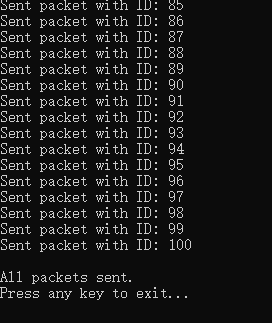
\includegraphics{img/sender.png}
        }
        \subcaption{发送端运行结果}
    \end{minipage}
    \hfill
    % 第二张图片
    \begin{minipage}[t]{0.48\textwidth}
        \centering
        \adjustbox{
            max width=0.73\linewidth,
            max height=0.55\textheight,
            min width=1cm,
            min height=1cm,
            keepaspectratio
        }{
            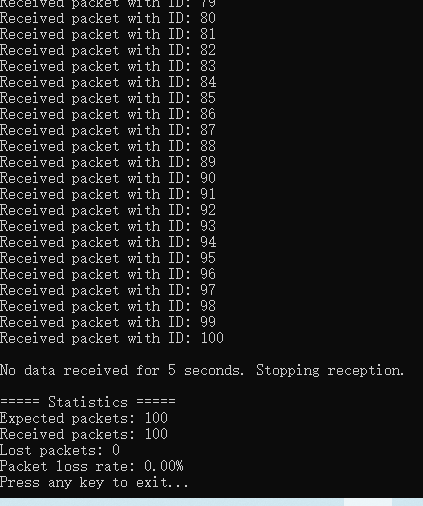
\includegraphics{img/receiver.png}
        }
        \subcaption{接收端运行结果}
    \end{minipage}
    \caption{发送端和接收端运行结果截图}
\end{figure}

从两张图可以看出，发送端成功发送了100个数据包，而接收端也成功接收了100个数据包，没有出现丢包现象。

同时，我们也保存了wireshark的抓包结果，分别如下所示：

\begin{figure}[H]
    \centering
    \adjustbox{
        max width=0.7\linewidth,
        max height=0.6\textheight,
        min width=1cm,
        min height=1cm,
        keepaspectratio
    }{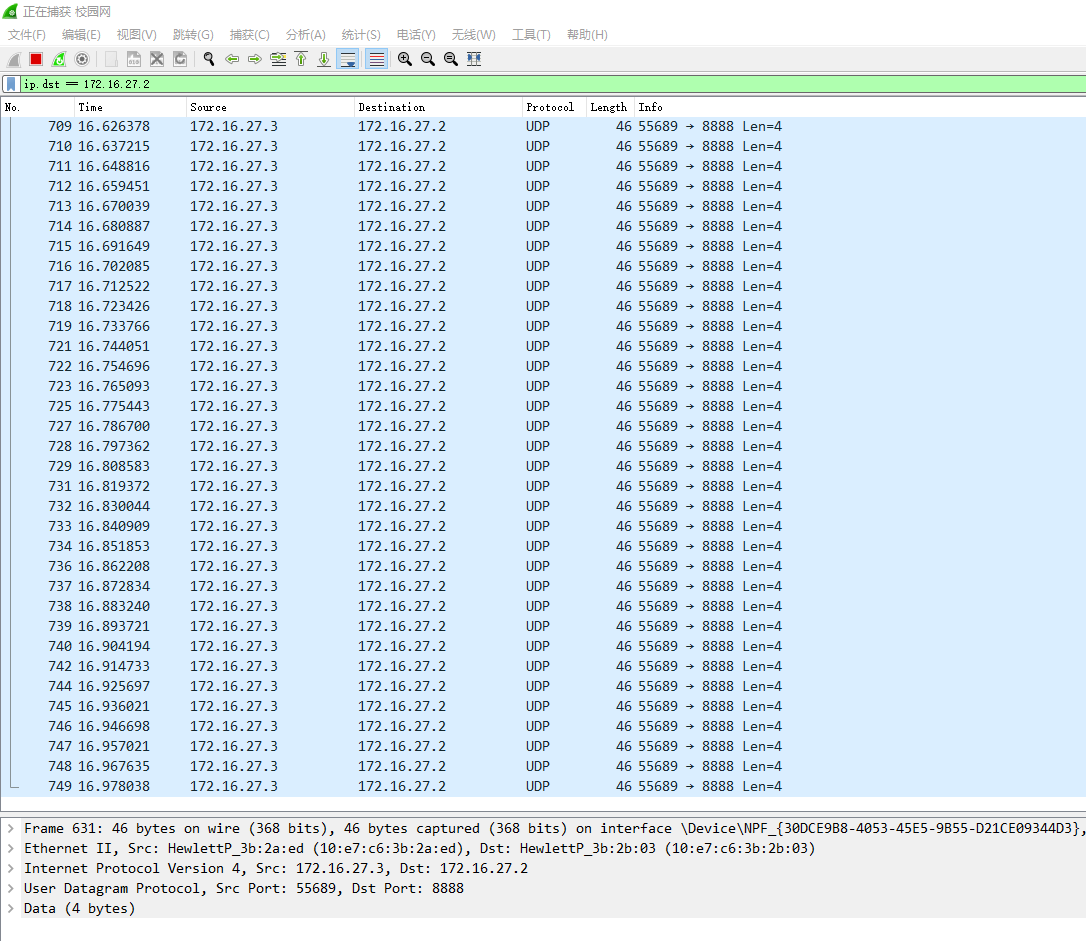
\includegraphics{img/sender_wireshark.png}}
    \caption{sender端抓包结果}
\end{figure}


\begin{figure}[H]
    \centering
    \adjustbox{
        max width=0.7\linewidth,
        max height=0.6\textheight,
        min width=1cm,
        min height=1cm,
        keepaspectratio
    }{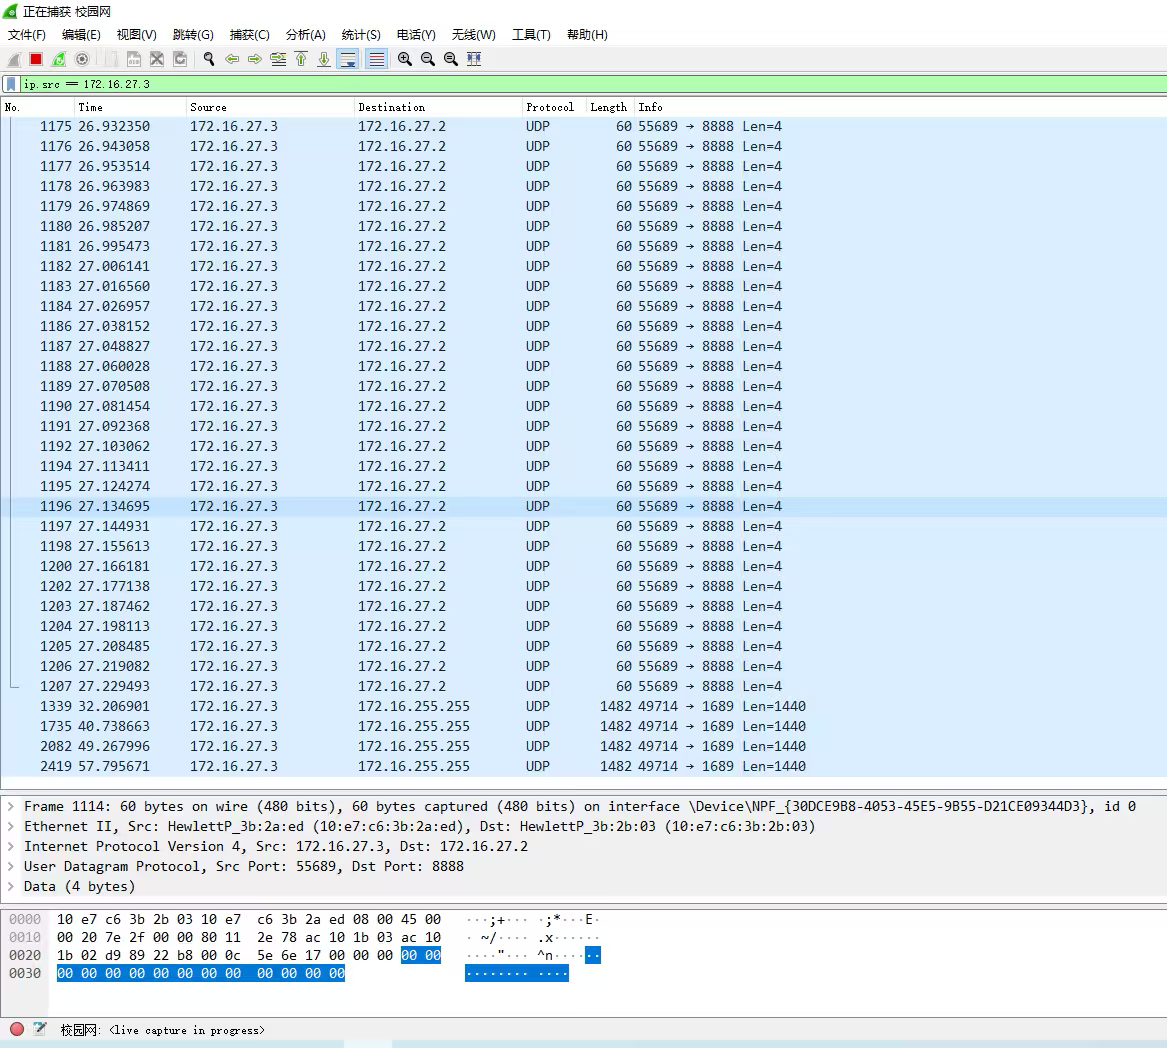
\includegraphics{img/receiver_wireshark.png}}
    \caption{receiver端抓包结果}
\end{figure}

这里wireshark抓包结果显示，发送端发送的UDP包确实到达了接收端，且包的源IP、目的IP和端口号均与我们程序中设置的一致。每个包的长度为8字节（4字节包ID + 4字节其他数据），符合预期。

\noindent\textbf{实验结果总结：}

本次实验通过在 sender 和 receiver 两台主机上分别使用 Wireshark 抓包，成功验证了数据包的发送与接收过程。实验结果显示，发送端成功发送了 100 个数据包，接收端也全部正确接收，未出现丢包现象。抓包结果进一步证明了数据包的源 IP、目的 IP 及端口号均与实验设置一致，数据传输过程稳定可靠，达到了预期实验目标。这说明本次网络通信程序设计正确，数据传输过程中的各项参数设置合理，能够满足实际应用需求。


\newpage

\section{实验思考题}

\subsection{程序流程图及关键函数说明}

根据程序的编写逻辑，我们绘制了发送端和接收端的程序流程图如下所示（这里用的mermaid flow chart 网站在线生图，好像有点小了，可以放大来看）：

\begin{figure}[H]
    \centering
    % 第一张图片
    \begin{minipage}[t]{0.4\textwidth}
        \centering
        \adjustbox{
            max width=1\linewidth,
            max height=0.5\textheight,
            min width=1cm,
            min height=1cm,
            keepaspectratio
        }{
            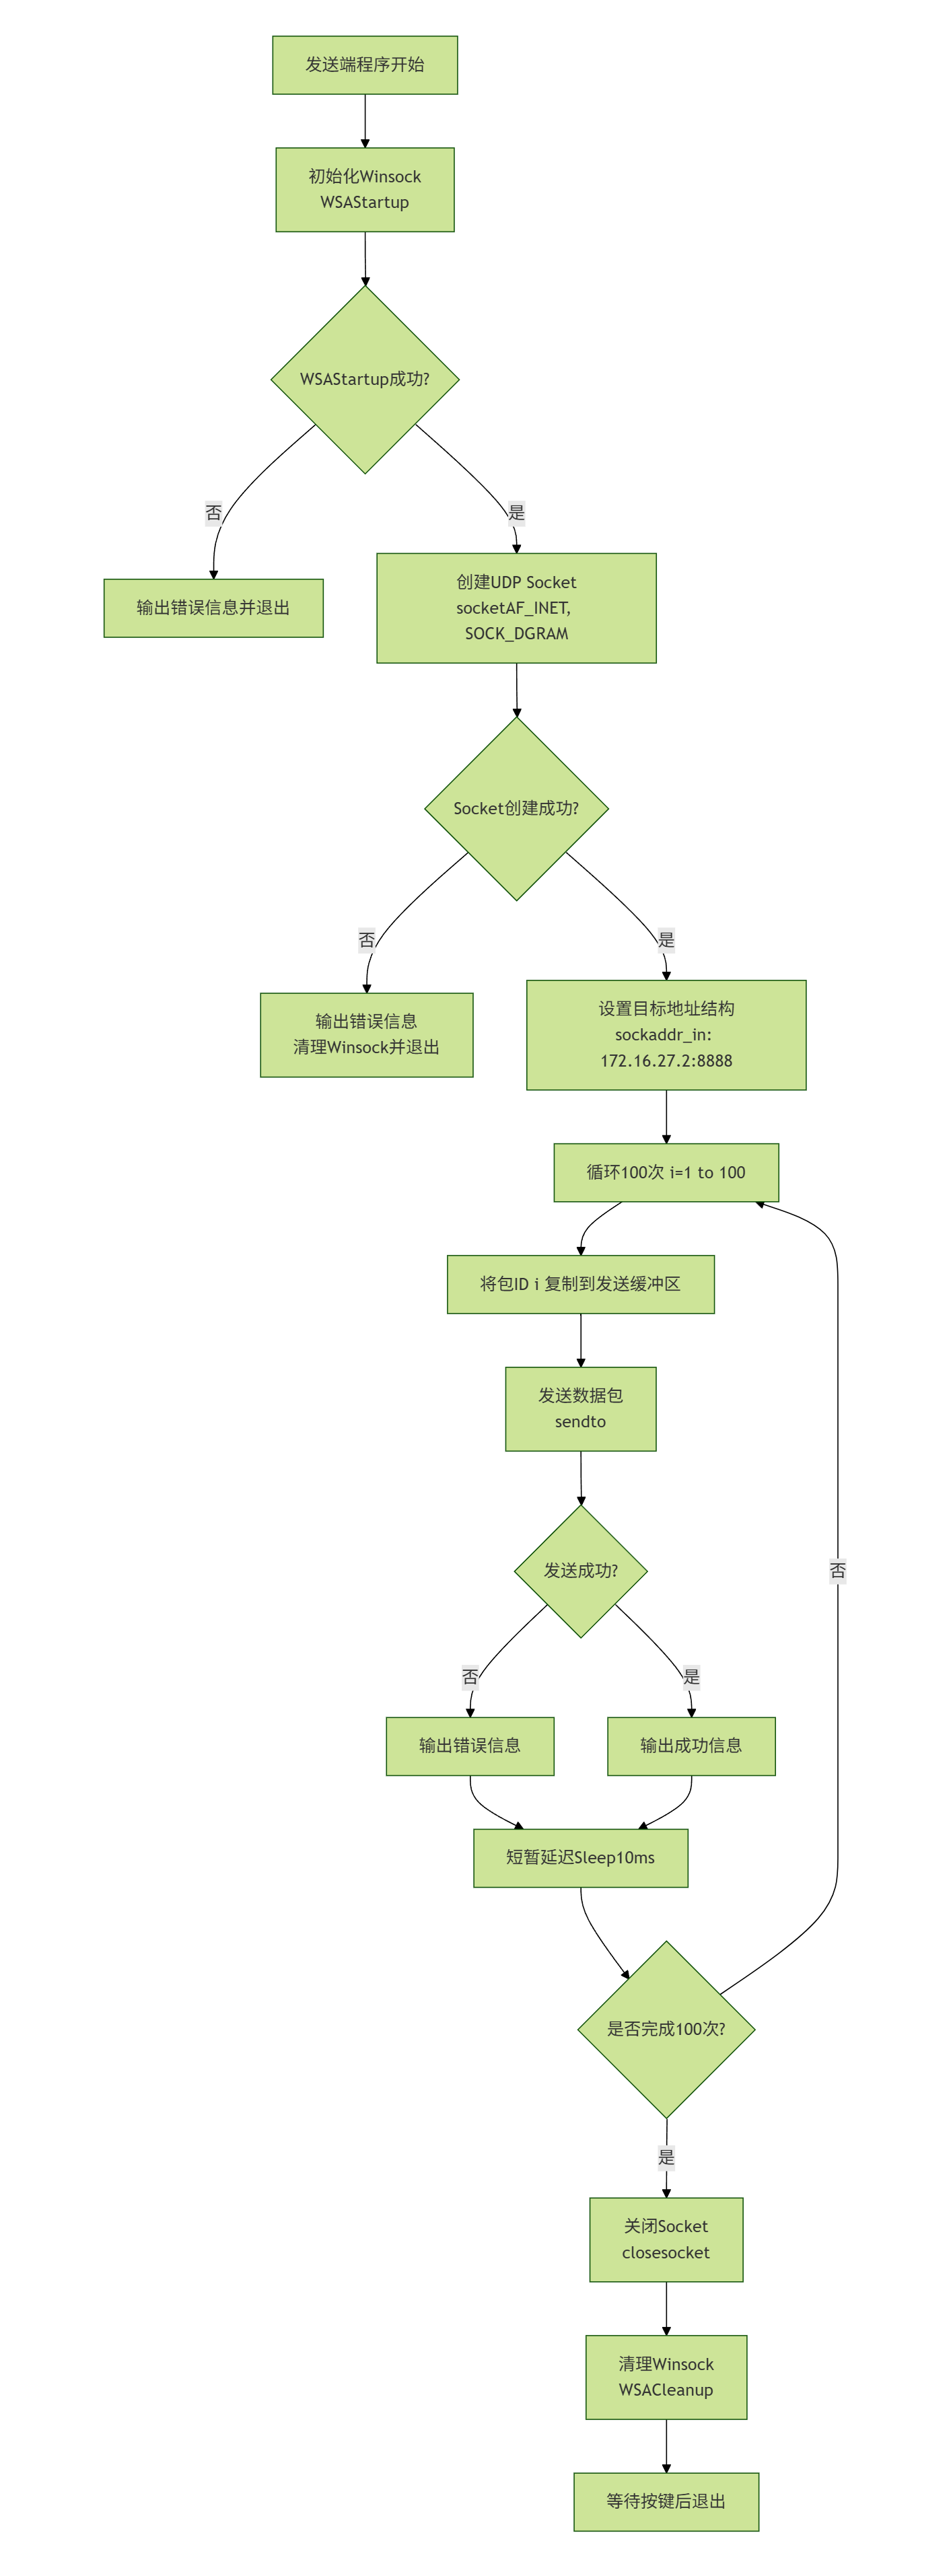
\includegraphics{img/sender_flow.png}
        }
        \subcaption{发送端运行流程图}
    \end{minipage}
    \hfill
    % 第二张图片
    \begin{minipage}[t]{0.58\textwidth}
        \centering
        \adjustbox{
            max width=1\linewidth,
            max height=0.8\textheight,
            min width=1cm,
            min height=1cm,
            keepaspectratio
        }{
            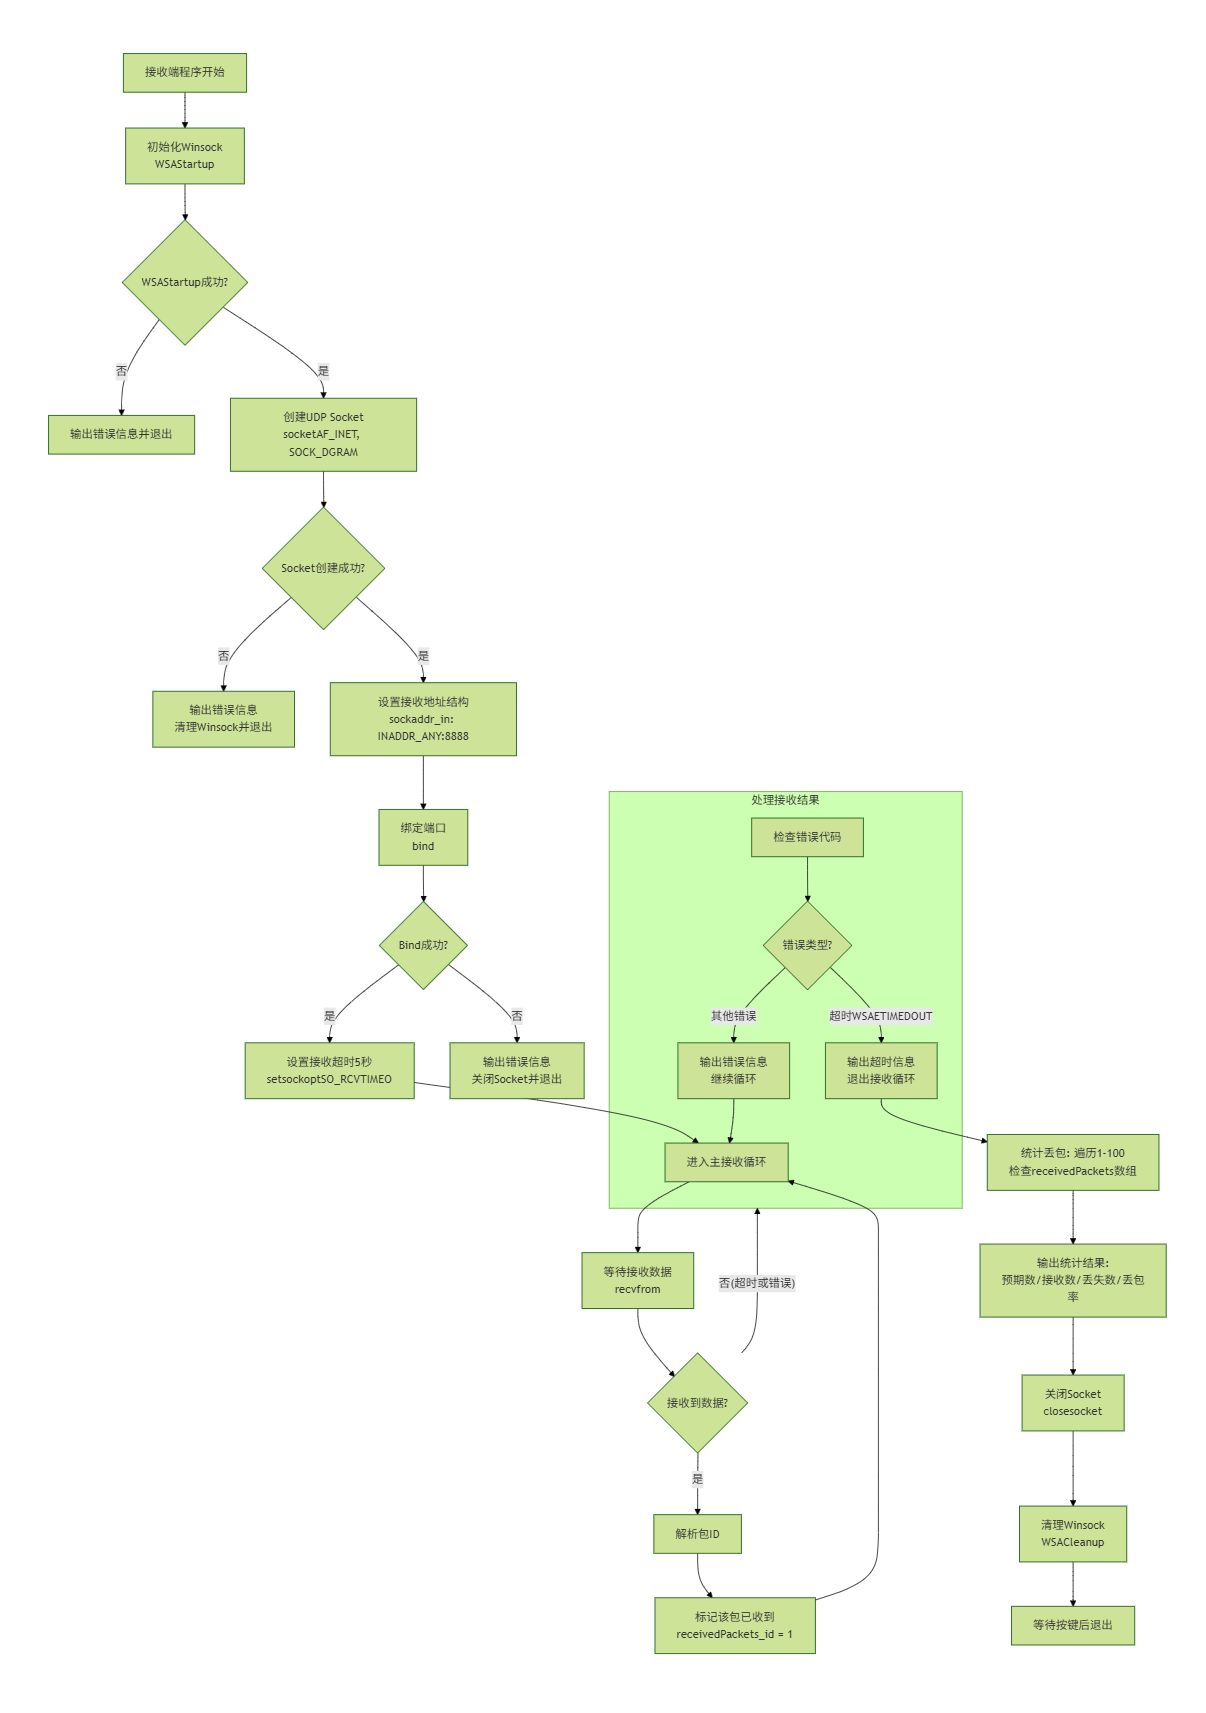
\includegraphics{img/receiver_flow.png}
        }
        \subcaption{接收端运行流程图}
    \end{minipage}
    \caption{发送端和接收端程序流程图}
\end{figure}

而流程实际上并不复杂，在前面放的那张示意图（图6）已经很清晰了，这里我们再用文字简单总结一下：

\noindent
\begin{minipage}[t]{0.48\textwidth}
\begin{myquote}
\textbf{发送端程序流程：}
\begin{enumerate}
    \item 初始化Winsock库
    \item 创建UDP套接字
    \item 设置目标地址结构
    \item 循环发送100个数据包
    \item 清理资源并退出
\end{enumerate}
\end{myquote}
\end{minipage}
\hfill
\begin{minipage}[t]{0.48\textwidth}
\begin{myquote}
\textbf{接收端程序流程：}
\begin{enumerate}
    \item 初始化Winsock库
    \item 创建UDP套接字
    \item 绑定本地地址和端口
    \item 设置接收超时时间
    \item 循环接收数据包并记录
    \item 统计丢包情况并输出结果
    \item 清理资源并退出
\end{enumerate}
\end{myquote}
\end{minipage}


\subsubsection{关键函数说明}

前面有提到过，这里就再简单总结一下程序中用到的关键函数及其作用：

\begin{itemize}
    \item \textbf{WSAStartup()}: 初始化Winsock库，必须在使用任何socket函数之前调用
    \item \textbf{socket()}: 创建套接字，参数AF\_INET表示IPv4，SOCK\_DGRAM表示UDP协议
    \item \textbf{bind()}: 仅接收端调用，将套接字绑定到本地地址和端口
    \item \textbf{sendto()}: 发送端用于发送数据包，包内容前4字节为包ID（int类型）
    \item \textbf{recvfrom()}: 接收端用于接收数据包，解析前4字节获得包ID
    \item \textbf{setsockopt()}: 接收端设置SO\_RCVTIMEO，超时时间为5秒，避免阻塞
    \item \textbf{Sleep()}: 发送端每发送一个包后延迟10ms，避免网络拥塞
    \item \textbf{统计丢包}: 接收端用 receivedPackets 数组标记收到的包，统计丢失包数量和丢包率
\end{itemize}


\subsection{struct sockaddr参数详解}

\begin{myquote}
\textbf{struct sockaddr\_in结构体各部分含义：}
\begin{itemize}
    \item \textbf{sin\_family}: 地址族，AF\_INET表示IPv4
    \item \textbf{sin\_port}: 端口号，发送端和接收端均为8888，需用htons()转换
    \item \textbf{sin\_addr.s\_addr}: IP地址，发送端目标为"172.16.27.2"，接收端为INADDR\_ANY
\end{itemize}

\textbf{具体示例：}
\begin{lstlisting}[language=C]
// 发送端
destAddr.sin_family = AF_INET;
destAddr.sin_port = htons(8888);
destAddr.sin_addr.s_addr = inet_addr("172.16.27.2");

// 接收端
recvAddr.sin_family = AF_INET;
recvAddr.sin_port = htons(8888);
recvAddr.sin_addr.s_addr = htonl(INADDR_ANY);
\end{lstlisting}
\end{myquote}

\subsection{面向连接与无连接Socket的区别}

\subsubsection{建立Socket时的区别}

\begin{table}[H]
    \centering
    \caption{建立Socket时的区别对比}
    \begin{tabular}{@{}p{0.15\textwidth}p{0.4\textwidth}p{0.4\textwidth}@{}}
        \toprule
        \textbf{特性} & \textbf{面向连接（TCP）} & \textbf{无连接（UDP）} \\
        \midrule
        创建套接字 & socket(AF\_INET, SOCK\_STREAM, IPPROTO\_TCP) & socket(AF\_INET, SOCK\_DGRAM, IPPROTO\_UDP) \\
        \midrule
        客户端连接 & 需要调用connect()建立连接 & 不需要建立连接，直接发送数据 \\
        \midrule
        服务器端等待 & 需要调用listen()和accept()等待连接 & 只需bind()绑定本地地址 \\
        \midrule
        连接状态 & 需要维护连接状态 & 无连接状态 \\
        \midrule
        资源开销 & 较高（连接维护） & 较低（无连接维护） \\
        \bottomrule
    \end{tabular}
\end{table}

\subsubsection{收发数据时的区别}

\begin{table}[H]
    \centering
    \caption{收发数据时的区别对比}
    \begin{tabular}{@{}p{0.15\textwidth}p{0.4\textwidth}p{0.4\textwidth}@{}}
        \toprule
        \textbf{特性} & \textbf{面向连接（TCP）} & \textbf{无连接（UDP）} \\
        \midrule
        发送函数 & send() & sendto()，每包前4字节为包ID \\
        \midrule
        接收函数 & recv() & recvfrom()，解析包ID \\
        \midrule
        地址指定 & 连接建立后不需要指定目标地址 & 每次发送都需指定目标地址 \\
        \midrule
        数据传输方式 & 数据流式传输，保证顺序和完整性 & 数据报式传输，不保证顺序和到达性 \\
        \midrule
        结束判断 & 通过连接关闭或特殊标记 & 接收端超时（5秒无数据）自动结束 \\
        \midrule
        可靠性 & 高（自动重传、确认） & 低（无重传机制） \\
        \bottomrule
    \end{tabular}
\end{table}

\subsection{面向连接与无连接通信的比较}

\begin{table}[H]
    \centering
    \caption{面向连接与无连接通信特性对比}
    \begin{tabular}{@{}p{0.12\textwidth}p{0.25\textwidth}p{0.25\textwidth}p{0.25\textwidth}@{}}
        \toprule
        \textbf{通信方式} & \textbf{优点} & \textbf{缺点} & \textbf{适用场合} \\
        \midrule
        \multirow{3}{*}{\textbf{TCP}} & 可靠性高，保证数据完整性和顺序 & 开销大，需要维护连接状态 & 文件传输 \\
        & 提供流量控制和拥塞控制 & 传输效率相对较低 & 网页浏览 \\
        & 自动重传丢失的数据 & 不适合实时性要求高的应用 & 电子邮件 \\
        \midrule
        \multirow{3}{*}{\textbf{UDP}} & 传输效率高，开销小 & 不保证数据可靠性 & 实时音视频传输 \\
        & 实时性好，延迟低 & 可能出现数据丢失、重复、乱序 & DNS查询 \\
        & 简单快速，无连接状态 & 无流量控制机制 & 在线游戏 \\
        \bottomrule
    \end{tabular}
\end{table}

\subsection{Socket工作方式分析}

本实验中Socket工作在\textbf{阻塞方式}。

\textbf{阻塞方式：}
\begin{itemize}
    \item recvfrom()函数会一直等待直到收到数据或超时
    \item 程序执行流会被挂起，等待I/O操作完成
    \item 简单易用，但可能导致程序响应性差
\end{itemize}

\textbf{非阻塞方式：}
\begin{itemize}
    \item I/O操作立即返回，不会阻塞程序执行
    \item 需要轮询或使用select/epoll等机制检查I/O状态
    \item 程序响应性好，但编程复杂度高
\end{itemize}

本实验通过设置SO\_RCVTIMEO选项实现了带超时的阻塞接收，在指定时间内没有数据时自动返回。

\subsection{UDP数据包丢失原因及解决方案}

\noindent
\begin{minipage}[t]{0.48\textwidth}
\begin{myquote}
\textbf{UDP数据包丢失的主要原因：}
\begin{itemize}
    \item \textbf{网络拥塞}: 网络带宽不足或路由器缓冲区溢出
    \item \textbf{接收缓冲区溢出}: 接收端处理速度跟不上发送速度
    \item \textbf{网络设备故障}: 交换机、路由器等设备出现问题
    \item \textbf{传输错误}: 物理链路传输过程中出现比特错误
    \item \textbf{发送速度过快}: 发送端发送频率超过网络承载能力
\end{itemize}
\end{myquote}
\end{minipage}
\hfill
\begin{minipage}[t]{0.48\textwidth}
\begin{myquote}
\textbf{解决方案：}
\begin{itemize}
    \item \textbf{应用层重传}: 实现ACK确认机制，超时重传丢失的包
    \item \textbf{流量控制}: 动态调整发送速率，避免网络拥塞
    \item \textbf{增大缓冲区}: 适当增大接收端缓冲区大小
    \item \textbf{数据包序号}: 添加序列号检测丢包和重复
    \item \textbf{错误检测与纠正}: 使用校验和、前向纠错等技术
    \item \textbf{冗余传输}: 关键数据多次发送或使用不同路径
\end{itemize}
\end{myquote}
\end{minipage}

\subsection{实验过程中遇到的问题及解决方法}

\textbf{遇到的主要问题：}
\begin{enumerate}
    \item \textbf{IP地址配置错误}: 初期设置的IP地址不在同一网段，导致无法通信
    \begin{itemize}
        \item 解决方法：重新配置IP地址为172.16.27.2和172.16.27.3，确保在同一网段
    \end{itemize}
    
    \item \textbf{防火墙阻止}: Windows防火墙阻止程序网络访问
    \begin{itemize}
        \item 解决方法：在防火墙中添加程序例外或临时关闭防火墙
    \end{itemize}
    
    \item \textbf{端口占用}: 8888端口被其他程序占用
    \begin{itemize}
        \item 解决方法：使用netstat命令检查端口占用情况，更换端口或终止占用程序
    \end{itemize}
    
    \item \textbf{接收超时设置}: 初期未设置接收超时，程序可能无限等待
    \begin{itemize}
        \item 解决方法：使用setsockopt()设置SO\_RCVTIMEO选项，避免程序永久阻塞
    \end{itemize}
\end{enumerate}


\subsection{实验思路总结}

\textbf{本实验的核心思路：}
\begin{enumerate}
    \item 设计发送端程序，连续发送100个带有序列号的UDP数据包
    \item 设计接收端程序，记录收到的数据包序列号并统计丢包情况
    \item 使用Wireshark抓包工具监控网络传输过程
    \item 通过对比发送和接收的数据包数量，分析网络传输的可靠性
    \item 深入理解UDP协议的特点和Socket编程的基本原理
\end{enumerate}

通过本实验，我们成功验证了UDP通信的基本原理，掌握了Socket编程的核心技术，并学会了使用网络分析工具进行数据包跟踪分析。实验结果表明，在良好的网络环境下，UDP传输是可靠的，但在实际应用中需要考虑各种可能导致丢包的因素。
\section{拓展试验一}

\subsection{实验目标与原理}

本拓展实验旨在深入理解TCP协议的工作原理，通过基于TCP套接字的数据通信实现多客户端聊天室功能。

\begin{myquote}
\textbf{实验核心原理：}
\begin{itemize}
    \item 使用TCP协议建立可靠的客户端-服务器连接
    \item 服务器支持多客户端同时连接，实现聊天室功能
    \item 通过线程技术处理并发连接和消息广播
    \item 使用Wireshark分析TCP三次握手和数据传输过程
\end{itemize}
\end{myquote}

TCP协议作为面向连接的可靠传输协议，与UDP的主要区别在于需要建立连接、保证数据顺序和完整性。本实验通过实现聊天室功能，深入体验TCP编程的特点。

\subsection{程序设计与实现}

\subsubsection{程序架构设计}

基于TCP的聊天室系统采用客户端-服务器架构，服务器端维护多个客户端连接，实现消息的接收和广播功能。

\begin{figure}[H]
    \centering
    \begin{tikzpicture}[node distance=2cm]
        % 服务器
        \node[rectangle, draw, fill=blue!20, minimum width=3cm, minimum height=1cm] (server) {TCP服务器};
        
        % 客户端
        \node[rectangle, draw, fill=green!20, minimum width=2cm, minimum height=0.8cm, above left=1cm and 2cm of server] (client1) {客户端1};
        \node[rectangle, draw, fill=green!20, minimum width=2cm, minimum height=0.8cm, left=3cm of server] (client2) {客户端2};
        \node[rectangle, draw, fill=green!20, minimum width=2cm, minimum height=0.8cm, below left=1cm and 2cm of server] (client3) {客户端3};
        
        % 连接线
        \draw[<->, thick] (client1) -- (server) node[midway, above, sloped] {TCP连接};
        \draw[<->, thick] (client2) -- (server) node[midway, above] {TCP连接};
        \draw[<->, thick] (client3) -- (server) node[midway, below, sloped] {TCP连接};
        
    \end{tikzpicture}
    \caption{TCP聊天室系统架构图}
\end{figure}

\subsubsection{服务器端核心代码}

服务器端的核心在于客户端管理和消息广播机制。我们使用线程池技术处理多客户端并发连接：

\begin{lstlisting}[language=C]
// 客户端信息结构
typedef struct {
    SOCKET socket;
    struct sockaddr_in addr;
    int id;
    char username[50];
    int active;
} ClientInfo;

// 全局变量
ClientInfo clients[MAX_CLIENTS];
int clientCount = 0;
CRITICAL_SECTION clientsLock;

// 主循环：接受客户端连接
while (1) {
    clientSocket = accept(serverSocket, (SOCKADDR*)&clientAddr, &clientAddrSize);
    if (clientSocket == INVALID_SOCKET) {
        printf("accept() failed with error %d\n", WSAGetLastError());
        continue;
    }
    
    // 添加新客户端
    int clientID = addClient(clientSocket, clientAddr);
    if (clientID == -1) {
        printf("服务器已满，拒绝连接 %s:%d\n", 
               inet_ntoa(clientAddr.sin_addr), ntohs(clientAddr.sin_port));
        closesocket(clientSocket);
        continue;
    }
    
    // 为每个客户端创建处理线程
    HANDLE hThread = (HANDLE)_beginthreadex(NULL, 0, handleClient, &clients[clientID], 0, NULL);
    // ...existing code...
}

// 广播消息给所有客户端
void broadcastMessage(char* message, int senderID) {
    EnterCriticalSection(&clientsLock);
    
    for (int i = 0; i < MAX_CLIENTS; i++) {
        if (clients[i].active && i != senderID) {
            if (send(clients[i].socket, message, strlen(message), 0) == SOCKET_ERROR) {
                printf("发送消息到客户端 %d 失败\n", clients[i].id);
            }
        }
    }
    
    LeaveCriticalSection(&clientsLock);
}
\end{lstlisting}

\subsubsection{客户端核心代码}

客户端程序相对简单，主要负责建立TCP连接和双向数据通信：

\begin{lstlisting}[language=C]
// 连接到服务器
if (connect(clientSocket, (SOCKADDR*)&serverAddr, sizeof(serverAddr)) == SOCKET_ERROR) {
    printf("连接服务器失败，错误代码: %d\n", WSAGetLastError());
    printf("请确保服务器正在运行并且IP地址正确\n");
    closesocket(clientSocket);
    WSACleanup();
    return 1;
}

printf("成功连接到服务器！\n\n");

// 创建接收消息的线程
HANDLE hReceiveThread = (HANDLE)_beginthreadex(NULL, 0, receiveMessages, NULL, 0, NULL);

// 主循环：发送消息
while (running) {
    printf("输入消息 (输入 'quit' 退出): ");
    if (fgets(sendBuffer, sizeof(sendBuffer), stdin) != NULL) {
        // 移除换行符
        char* newline = strchr(sendBuffer, '\n');
        if (newline) *newline = '\0';
        
        // 检查是否要退出
        if (strcmp(sendBuffer, "quit") == 0) {
            running = 0;
            break;
        }
        
        // 发送消息到服务器
        if (send(clientSocket, sendBuffer, strlen(sendBuffer), 0) == SOCKET_ERROR) {
            printf("发送消息失败，错误代码: %d\n", WSAGetLastError());
            running = 0;
            break;
        }
    }
}
\end{lstlisting}

\subsubsection{统一主程序设计}

为了便于测试和演示，我们设计了统一的主程序，可以选择运行服务器或客户端模式：

\begin{lstlisting}[language=C]
int main() {
    int choice;
    
    printf("==========================================================\n");
    printf("            TCP套接字数据通信实验程序\n");
    printf("==========================================================\n");
    printf("实验功能:\n");
    printf("1. 基于TCP协议的客户端-服务器通信\n");
    printf("2. 支持多客户端同时连接\n");
    printf("3. 实现聊天室功能和数据交互\n");
    printf("4. 可用Wireshark分析网络数据包\n");
    printf("==========================================================\n\n");
    
    printf("请选择运行模式:\n");
    printf("1. 运行TCP服务器\n");
    printf("2. 运行TCP客户端\n");
    printf("3. 退出程序\n");
    printf("\n请输入选择 (1-3): ");
    
    scanf("%d", &choice);
    
    switch (choice) {
        case 1: runServer(); break;
        case 2: runClient(); break;
        case 3: printf("\n程序退出。\n"); break;
        default: printf("\n无效选择，程序退出。\n"); break;
    }
    
    return 0;
}
\end{lstlisting}

\subsection{实验步骤与结果}

\subsubsection{实验环境配置}

按照主实验的网络配置，我们继续使用2号机（172.16.27.2）作为服务器，3号机（172.16.27.3）作为客户端进行测试。

\subsubsection{程序运行过程}

\textbf{Step 1}: 编译程序并启动Wireshark监控
\begin{lstlisting}[language=bash]
gcc -o extend.exe extend.c -lws2_32
\end{lstlisting}

\textbf{Step 2}: 在2号机上启动服务器程序，选择模式1\\

\textbf{Step 3}: 在3号机上启动客户端程序，选择模式2\\

\textbf{Step 4}: 进行聊天测试并观察数据包传输

\subsubsection{实验结果展示}

\begin{figure}[H]
    \centering
    % 第一张图片
    \begin{minipage}[t]{0.48\textwidth}
        \centering
        \adjustbox{
            max width=1\linewidth,
            max height=0.45\textheight,
            min width=1cm,
            min height=1cm,
            keepaspectratio
        }{
            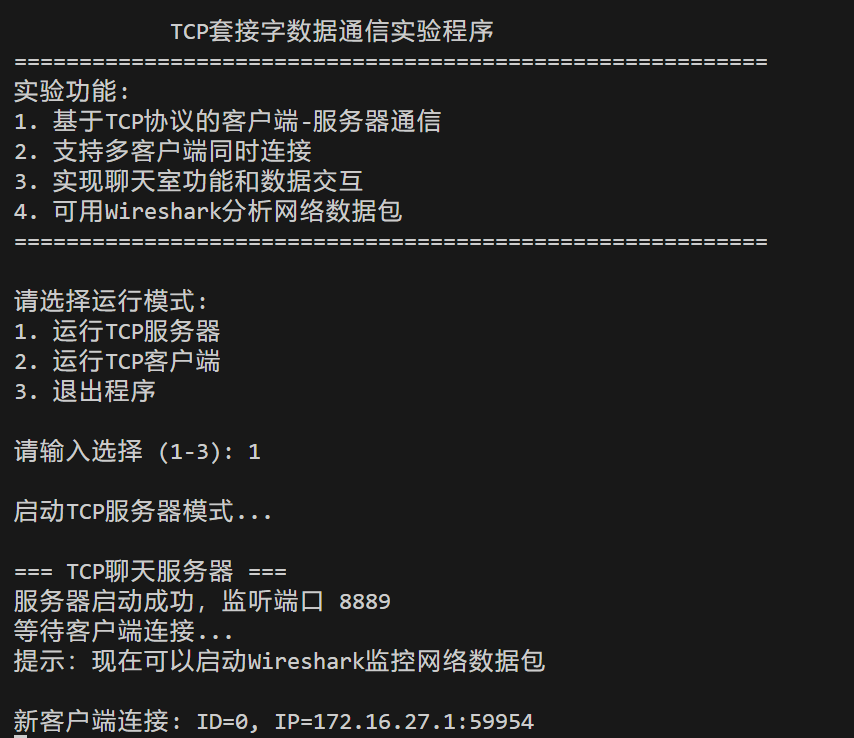
\includegraphics{img/extend_lab/tcp_server_running.png}
        }
        \subcaption{TCP服务器运行界面}
    \end{minipage}
    \hfill
    % 第二张图片
    \begin{minipage}[t]{0.48\textwidth}
        \centering
        \adjustbox{
            max width=1\linewidth,
            max height=0.45\textheight,
            min width=1cm,
            min height=1cm,
            keepaspectratio
        }{
            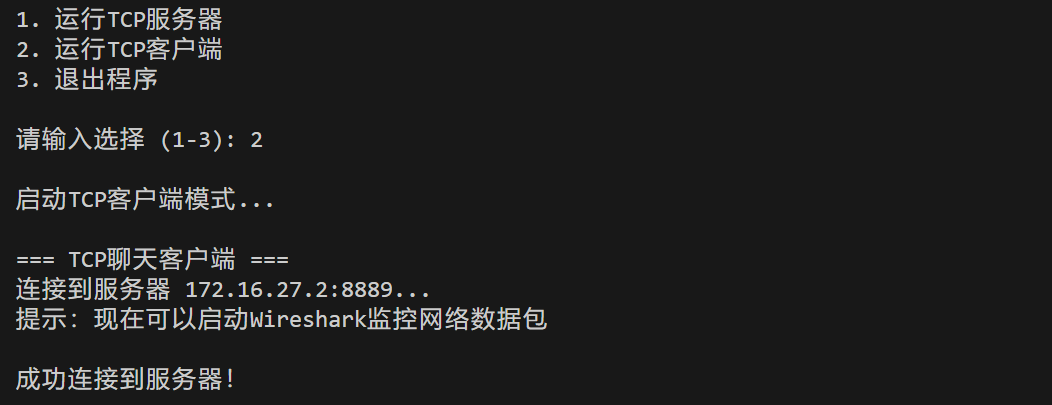
\includegraphics{img/extend_lab/tcp_client_running.png}
        }
        \subcaption{TCP客户端运行界面}
    \end{minipage}
    \caption{TCP聊天室程序运行截图}
\end{figure}

\begin{figure}[H]
    \centering
    % 第一张图片
    \begin{minipage}[t]{0.48\textwidth}
        \centering
        \adjustbox{
            max width=1\linewidth,
            max height=0.6\textheight,
            min width=1cm,
            min height=1cm,
            keepaspectratio
        }{
            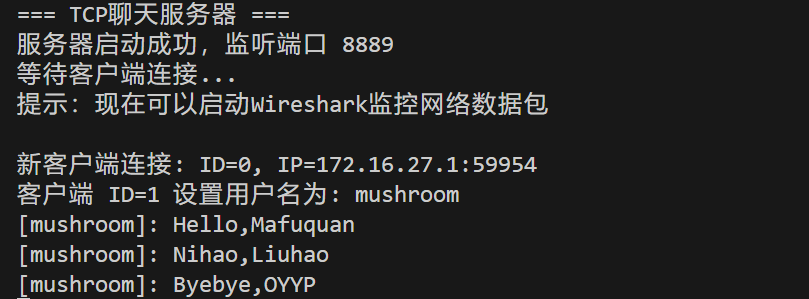
\includegraphics{img/extend_lab/tcp_chat_demo_server.png}
        }
        \subcaption{服务器端聊天演示}
    \end{minipage}
    \hfill
    % 第二张图片
    \begin{minipage}[t]{0.48\textwidth}
        \centering
        \adjustbox{
            max width=1\linewidth,
            max height=0.6\textheight,
            min width=1cm,
            min height=1cm,
            keepaspectratio
        }{
            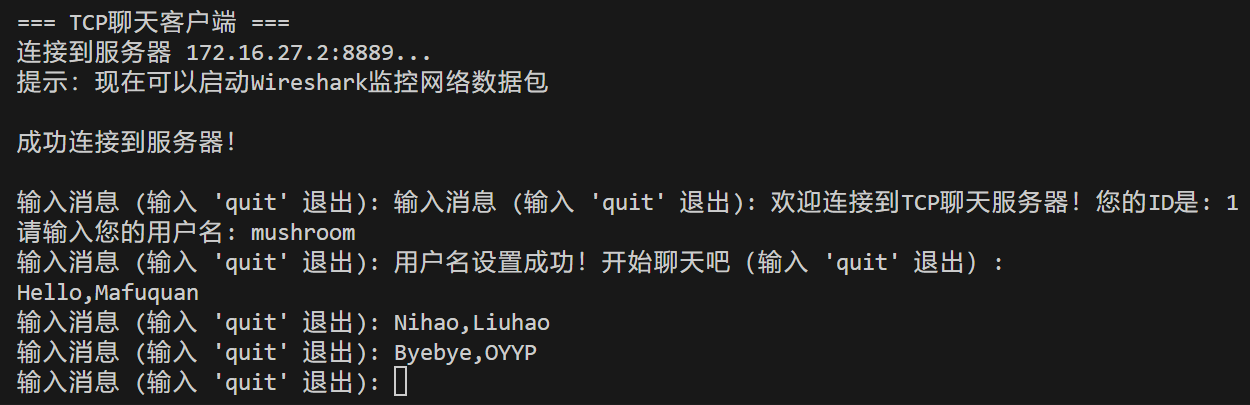
\includegraphics{img/extend_lab/tcp_chat_demo_client.png}
        }
        \subcaption{客户端聊天演示}
    \end{minipage}
    \caption{多客户端聊天演示}
\end{figure}

\subsection{Wireshark数据包分析}

\subsubsection{TCP三次握手分析}

通过Wireshark抓包，我们可以清晰地观察到TCP建立连接的三次握手过程：

\begin{figure}[H]
    \centering
    % 第一张图片
    \begin{minipage}[t]{0.48\textwidth}
        \centering
        \adjustbox{
            max width=1\linewidth,
            max height=0.6\textheight,
            min width=1cm,
            min height=1cm,
            keepaspectratio
        }{
            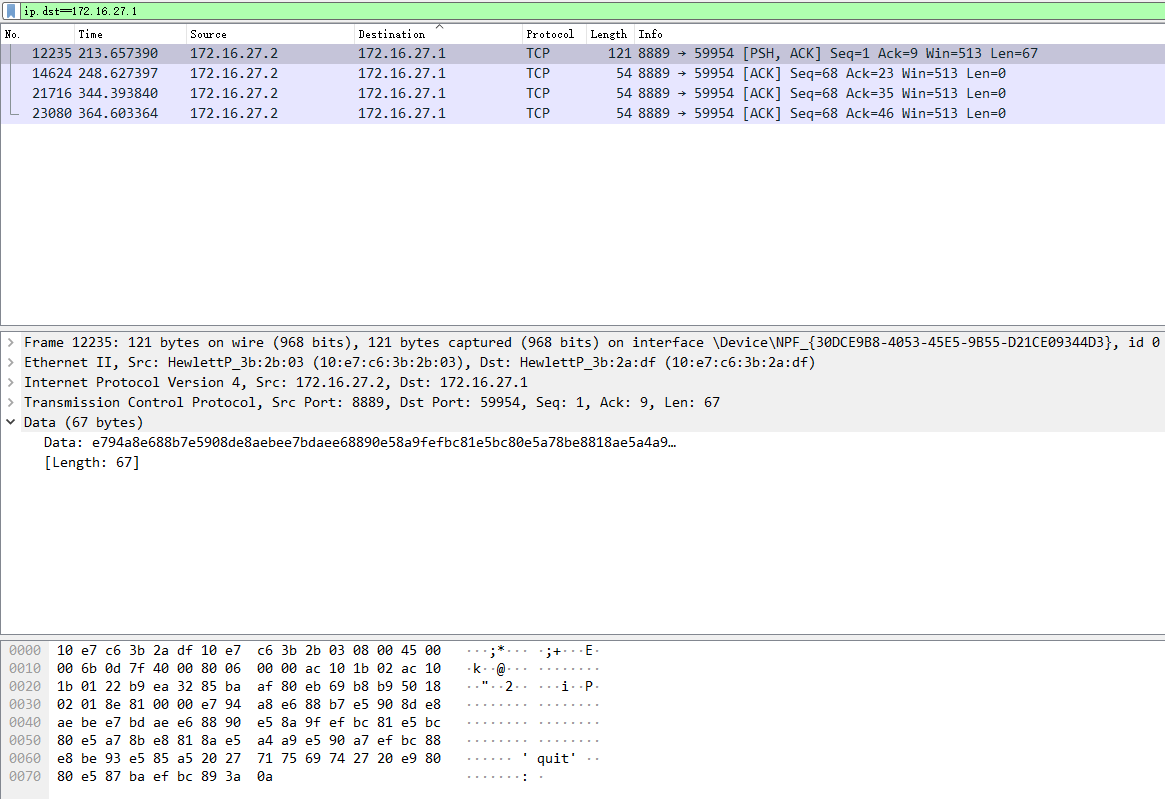
\includegraphics{img/extend_lab/server_wireshark.png}
        }
        \subcaption{服务器端抓包结果}
    \end{minipage}
    \hfill
    % 第二张图片
    \begin{minipage}[t]{0.48\textwidth}
        \centering
        \adjustbox{
            max width=1\linewidth,
            max height=0.6\textheight,
            min width=1cm,
            min height=1cm,
            keepaspectratio
        }{
            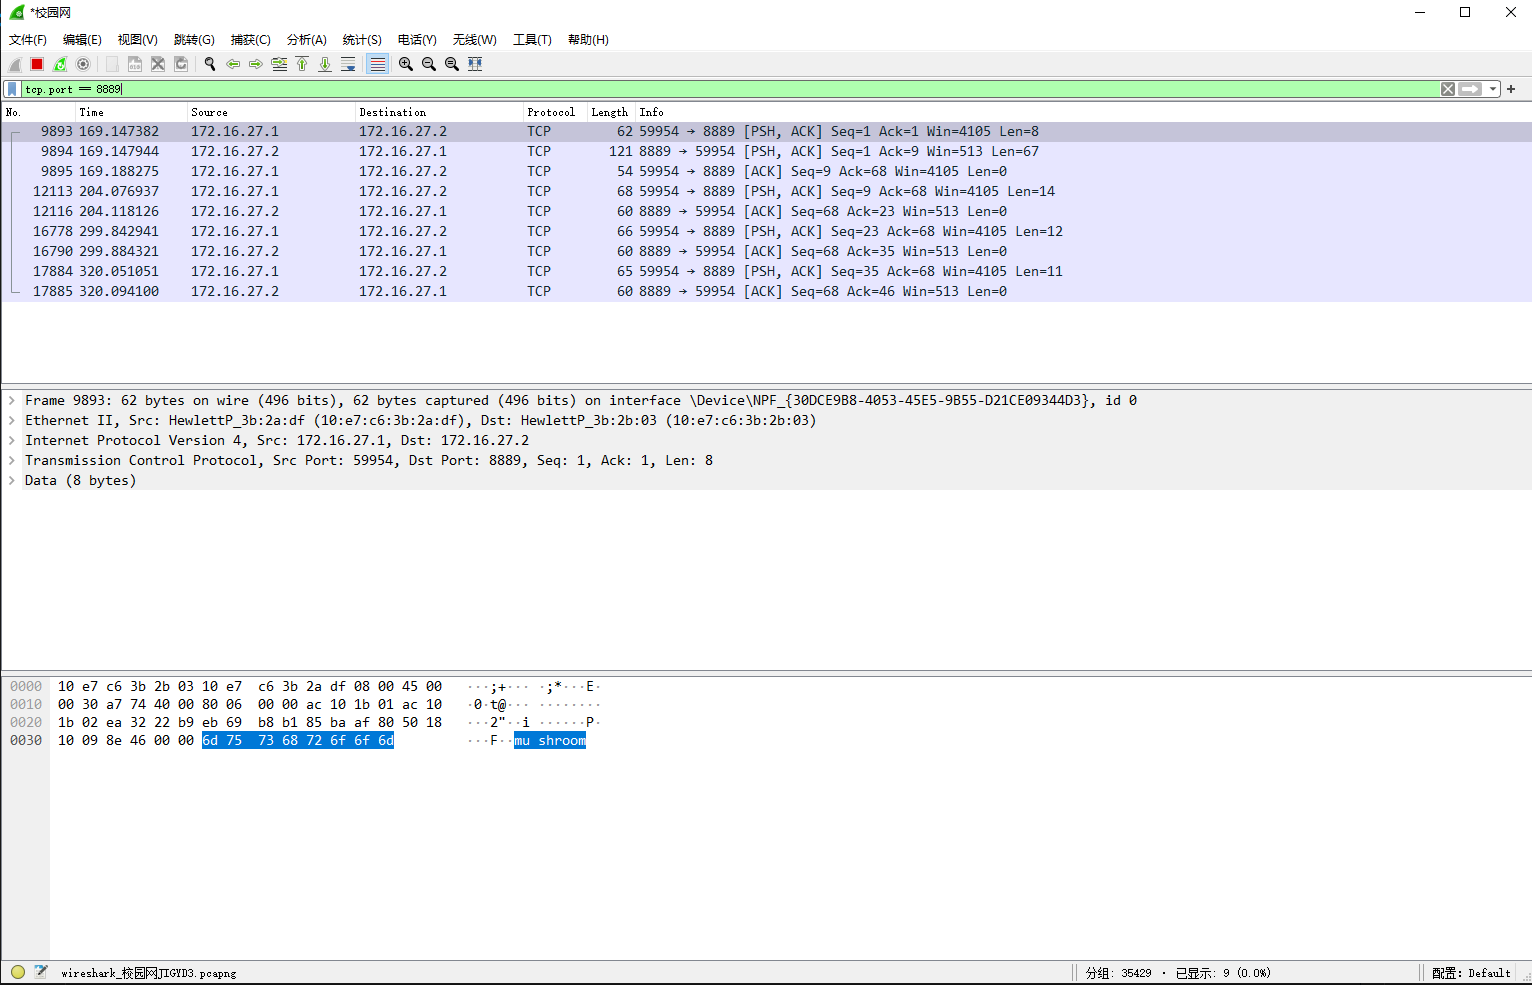
\includegraphics{img/extend_lab/client_wireshark.png}
        }
        \subcaption{客户端抓包结果}
    \end{minipage}
    \caption{TCP通信过程Wireshark抓包分析}
\end{figure}

\begin{table}[H]
    \centering
    \caption{TCP三次握手过程分析}
    \begin{tabular}{@{}cccc@{}}
        \toprule
        \textbf{步骤} & \textbf{包类型} & \textbf{源端口} & \textbf{目标端口} \\
        \midrule
        1 & SYN & 客户端随机端口 & 8889 \\
        2 & SYN-ACK & 8889 & 客户端端口 \\
        3 & ACK & 客户端端口 & 8889 \\
        \bottomrule
    \end{tabular}
\end{table}

\subsubsection{数据传输与连接断开过程分析}

从Wireshark抓包结果可以看出，TCP协议的完整通信过程包括：

\begin{itemize}
    \item \textbf{连接建立}: 客户端发送SYN包请求连接，服务器响应SYN-ACK包，客户端确认ACK完成三次握手
    \item \textbf{数据传输}: 聊天消息通过PSH-ACK包进行传输，每个数据包都有序列号和确认号
    \item \textbf{连接断开}: 当客户端输入"quit"命令时，执行四次挥手断开连接
    \item \textbf{可靠性保证}: 接收方对每个数据包都进行ACK确认，确保数据传输的可靠性
\end{itemize}

通过对比服务器端和客户端的抓包结果，我们可以验证TCP协议的双向通信机制和可靠传输特性，为理解网络协议工作原理提供了直观的实验证据。

% ...existing code...
\begin{thebibliography}{99}  

    \bibitem{ref1}Yi Xie. (2025). 中山大学计算机网络实验课程.
    \bibitem{ref2}WEB. (N.A.). 互联网内容.
    \bibitem{ref3}CSDN博客. (2023). socket技术详解. \url{https://blog.csdn.net/fuhanghang/article/details/114528098}

\end{thebibliography}


\end{document}